% Options for packages loaded elsewhere
\PassOptionsToPackage{unicode}{hyperref}
\PassOptionsToPackage{hyphens}{url}
\PassOptionsToPackage{dvipsnames,svgnames,x11names}{xcolor}
%
\documentclass[
  article]{jss}

\usepackage{amsmath,amssymb}
\usepackage{iftex}
\ifPDFTeX
  \usepackage[T1]{fontenc}
  \usepackage[utf8]{inputenc}
  \usepackage{textcomp} % provide euro and other symbols
\else % if luatex or xetex
  \usepackage{unicode-math}
  \defaultfontfeatures{Scale=MatchLowercase}
  \defaultfontfeatures[\rmfamily]{Ligatures=TeX,Scale=1}
\fi
\usepackage{lmodern}
\ifPDFTeX\else  
    % xetex/luatex font selection
\fi
% Use upquote if available, for straight quotes in verbatim environments
\IfFileExists{upquote.sty}{\usepackage{upquote}}{}
\IfFileExists{microtype.sty}{% use microtype if available
  \usepackage[]{microtype}
  \UseMicrotypeSet[protrusion]{basicmath} % disable protrusion for tt fonts
}{}
\makeatletter
\@ifundefined{KOMAClassName}{% if non-KOMA class
  \IfFileExists{parskip.sty}{%
    \usepackage{parskip}
  }{% else
    \setlength{\parindent}{0pt}
    \setlength{\parskip}{6pt plus 2pt minus 1pt}}
}{% if KOMA class
  \KOMAoptions{parskip=half}}
\makeatother
\usepackage{xcolor}
\setlength{\emergencystretch}{3em} % prevent overfull lines
\setcounter{secnumdepth}{-\maxdimen} % remove section numbering
% Make \paragraph and \subparagraph free-standing
\ifx\paragraph\undefined\else
  \let\oldparagraph\paragraph
  \renewcommand{\paragraph}[1]{\oldparagraph{#1}\mbox{}}
\fi
\ifx\subparagraph\undefined\else
  \let\oldsubparagraph\subparagraph
  \renewcommand{\subparagraph}[1]{\oldsubparagraph{#1}\mbox{}}
\fi


\providecommand{\tightlist}{%
  \setlength{\itemsep}{0pt}\setlength{\parskip}{0pt}}\usepackage{longtable,booktabs,array}
\usepackage{calc} % for calculating minipage widths
% Correct order of tables after \paragraph or \subparagraph
\usepackage{etoolbox}
\makeatletter
\patchcmd\longtable{\par}{\if@noskipsec\mbox{}\fi\par}{}{}
\makeatother
% Allow footnotes in longtable head/foot
\IfFileExists{footnotehyper.sty}{\usepackage{footnotehyper}}{\usepackage{footnote}}
\makesavenoteenv{longtable}
\usepackage{graphicx}
\makeatletter
\def\maxwidth{\ifdim\Gin@nat@width>\linewidth\linewidth\else\Gin@nat@width\fi}
\def\maxheight{\ifdim\Gin@nat@height>\textheight\textheight\else\Gin@nat@height\fi}
\makeatother
% Scale images if necessary, so that they will not overflow the page
% margins by default, and it is still possible to overwrite the defaults
% using explicit options in \includegraphics[width, height, ...]{}
\setkeys{Gin}{width=\maxwidth,height=\maxheight,keepaspectratio}
% Set default figure placement to htbp
\makeatletter
\def\fps@figure{htbp}
\makeatother

\usepackage{orcidlink,thumbpdf,lmodern}

\newcommand{\class}[1]{`\code{#1}'}
\newcommand{\fct}[1]{\code{#1()}}
\makeatletter
\@ifpackageloaded{tcolorbox}{}{\usepackage[skins,breakable]{tcolorbox}}
\@ifpackageloaded{fontawesome5}{}{\usepackage{fontawesome5}}
\definecolor{quarto-callout-color}{HTML}{909090}
\definecolor{quarto-callout-note-color}{HTML}{0758E5}
\definecolor{quarto-callout-important-color}{HTML}{CC1914}
\definecolor{quarto-callout-warning-color}{HTML}{EB9113}
\definecolor{quarto-callout-tip-color}{HTML}{00A047}
\definecolor{quarto-callout-caution-color}{HTML}{FC5300}
\definecolor{quarto-callout-color-frame}{HTML}{acacac}
\definecolor{quarto-callout-note-color-frame}{HTML}{4582ec}
\definecolor{quarto-callout-important-color-frame}{HTML}{d9534f}
\definecolor{quarto-callout-warning-color-frame}{HTML}{f0ad4e}
\definecolor{quarto-callout-tip-color-frame}{HTML}{02b875}
\definecolor{quarto-callout-caution-color-frame}{HTML}{fd7e14}
\makeatother
\makeatletter
\@ifpackageloaded{caption}{}{\usepackage{caption}}
\AtBeginDocument{%
\ifdefined\contentsname
  \renewcommand*\contentsname{Table of contents}
\else
  \newcommand\contentsname{Table of contents}
\fi
\ifdefined\listfigurename
  \renewcommand*\listfigurename{List of Figures}
\else
  \newcommand\listfigurename{List of Figures}
\fi
\ifdefined\listtablename
  \renewcommand*\listtablename{List of Tables}
\else
  \newcommand\listtablename{List of Tables}
\fi
\ifdefined\figurename
  \renewcommand*\figurename{Figure}
\else
  \newcommand\figurename{Figure}
\fi
\ifdefined\tablename
  \renewcommand*\tablename{Table}
\else
  \newcommand\tablename{Table}
\fi
}
\@ifpackageloaded{float}{}{\usepackage{float}}
\floatstyle{ruled}
\@ifundefined{c@chapter}{\newfloat{codelisting}{h}{lop}}{\newfloat{codelisting}{h}{lop}[chapter]}
\floatname{codelisting}{Listing}
\newcommand*\listoflistings{\listof{codelisting}{List of Listings}}
\makeatother
\makeatletter
\makeatother
\makeatletter
\@ifpackageloaded{caption}{}{\usepackage{caption}}
\@ifpackageloaded{subcaption}{}{\usepackage{subcaption}}
\makeatother
\makeatletter
\@ifpackageloaded{tcolorbox}{}{\usepackage[skins,breakable]{tcolorbox}}
\makeatother
\makeatletter
\@ifundefined{shadecolor}{\definecolor{shadecolor}{rgb}{.97, .97, .97}}{}
\makeatother
\makeatletter
\makeatother
\makeatletter
\ifdefined\Shaded\renewenvironment{Shaded}{\begin{tcolorbox}[frame hidden, boxrule=0pt, sharp corners, borderline west={3pt}{0pt}{shadecolor}, enhanced, interior hidden, breakable]}{\end{tcolorbox}}\fi
\makeatother
\ifLuaTeX
  \usepackage{selnolig}  % disable illegal ligatures
\fi
\usepackage{bookmark}

\IfFileExists{xurl.sty}{\usepackage{xurl}}{} % add URL line breaks if available
\urlstyle{same} % disable monospaced font for URLs
\hypersetup{
  pdftitle={A Short Demo Article: Regression Models for Count Data in R},
  pdfauthor={Achim Zeileis; Second Author},
  pdfkeywords={JSS, style guide, comma-separated, not capitalized, R},
  colorlinks=true,
  linkcolor={blue},
  filecolor={Maroon},
  citecolor={Blue},
  urlcolor={Blue},
  pdfcreator={LaTeX via pandoc}}

%% -- Article metainformation (author, title, ...) -----------------------------

%% Author information
\author{Achim Zeileis~\orcidlink{0000-0003-0918-3766}\\Universität
Innsbruck \And Second Author\\Plus Affiliation}
\Plainauthor{Achim Zeileis, Second Author} %% comma-separated

\title{A Short Demo Article: Regression Models for Count Data in R}
\Plaintitle{A Short Demo Article: Regression Models for Count Data in
R} %% without formatting

%% an abstract and keywords
\Abstract{This short article illustrates how to write a manuscript for
the \emph{Journal of Statistical Software} (JSS) using its {\LaTeX}
style files. Generally, we ask to follow JSS's style guide and FAQs
precisely. Also, it is recommended to keep the {\LaTeX} code as simple
as possible, i.e., avoid inclusion of packages/commands that are not
necessary. For outlining the typical structure of a JSS article some
brief text snippets are employed that have been inspired by
\citet{ZeileisKleiberJackman2008}, discussing count data regression in
\proglang{R}. Editorial comments and instructions are marked by vertical
bars.}

%% at least one keyword must be supplied
\Keywords{JSS, style guide, comma-separated, not
capitalized, \proglang{R}}
\Plainkeywords{JSS, style guide, comma-separated, not capitalized, R}

%% publication information
%% NOTE: Typically, this can be left commented and will be filled out by the technical editor
%% \Volume{50}
%% \Issue{9}
%% \Month{June}
%% \Year{2012}
%% \Submitdate{2012-06-04}
%% \Acceptdate{2012-06-04}
%% \setcounter{page}{1}
%% \Pages{1--xx}

%% The address of (at least) one author should be given
%% in the following format:
\Address{
Achim Zeileis\\
Department of Statistics\\
Universitätsstr. 15\\
Innsbruck Austria\\
E-mail: \email{Achim.Zeileis@R-project.org}\\
URL: \url{https://www.zeileis.org/}\\
\\~
Second Author\\
\\~

}

\begin{document}
\maketitle

\section{Introduction: Count data regression in R}\label{sec-intro}

\begin{tcolorbox}[enhanced jigsaw, colframe=quarto-callout-color-frame, leftrule=.75mm, breakable, left=2mm, bottomrule=.15mm, toprule=.15mm, opacityback=0, colback=white, arc=.35mm, rightrule=.15mm]

The introduction is in principle ``as usual''. However, it should
usually embed both the implemented \emph{methods} and the
\emph{software} into the respective relevant literature. For the latter
both competing and complementary software should be discussed (within
the same software environment and beyond), bringing out relative
(dis)advantages. All software mentioned should be properly
\texttt{@cited}'d.~(See also \hyperref[sec-bibtex]{Using BibTeX} for
more details on \textsc{Bib}{\TeX}.)

For writing about software JSS requires authors to use the markup
\texttt{{[}{]}\{.proglang\}} (programming languages and large
programmable systems), \texttt{{[}{]}\{.pkg\}} (software packages), back
ticks like `code` for code (functions, commands, arguments, etc.).

If there is such markup in (sub)section titles (as above), a plain text
version has to be provided in the {\LaTeX} command as well. Below we
also illustrate how abbrevations should be introduced and citation
commands can be employed. See the {\LaTeX} code for more details.

\end{tcolorbox}

Modeling count variables is a common task in economics and the social
sciences. The classical Poisson regression model for count data is often
of limited use in these disciplines because empirical count data sets
typically exhibit overdispersion and/or an excess number of zeros. The
former issue can be addressed by extending the plain Poisson regression
model in various directions: e.g., using sandwich covariances or
estimating an additional dispersion parameter (in a so-called
quasi-Poisson model). Another more formal way is to use a negative
binomial (NB) regression. All of these models belong to the family of
generalized linear models (GLMs). However, although these models
typically can capture overdispersion rather well, they are in many
applications not sufficient for modeling excess zeros. Since
\citet{Mullahy1986} there is increased interest in zero-augmented models
that address this issue by a second model component capturing zero
counts. An overview of count data models in econometrics, including
hurdle and zero-inflated models, is provided in
\citet{CameronTrivedi2013}.

In \proglang{R} \citet{R}, GLMs are provided by the model fitting
functions \fct{glm} in the \pkg{stats} package and \fct{glm.nb} in the
\pkg{MASS} package \citep{VenablesRipley2002} along with associated
methods for diagnostics and inference. The manuscript that this document
is based on \citep{ZeileisKleiberJackman2008} then introduced hurdle and
zero-inflated count models in the functions \fct{hurdle} and
\fct{zeroinfl} in the \pkg{pcsl} package \citet{Jackman2015}. Of course,
much more software could be discussed here, including (but not limited
to) generalized additive models for count data as available in the
\proglang{R} packages \pkg{mgcv} \citet{Wood2006}, \pkg{gamlss}
\citet{StasinopoulosRigby2007}, or \pkg{VGAM} \citet{Yee2009}.

\section{Models and software}\label{sec-models}

The basic Poisson regression model for count data is a special case of
the GLM framework \citet{McCullaghNelder1989}. It describes the
dependence of a count response variable \(y_i\) (\(i = 1, \dots, n\)) by
assuming a Poisson distribution \(y_i \sim \mathrm{Pois}(\mu_i)\). The
dependence of the conditional mean \(E[y_i \, | \, x_i] = \mu_i\) on the
regressors \(x_i\) is then specified via a log link and a linear
predictor

\begin{equation}\phantomsection\label{eq-mean}{
\log(\mu_i) \quad = \quad x_i^\top \beta,
}\end{equation}

where the regression coefficients \(\beta\) are estimated by maximum
likelihood (ML) using the iterative weighted least squares (IWLS)
algorithm.

\begin{tcolorbox}[enhanced jigsaw, colframe=quarto-callout-color-frame, leftrule=.75mm, breakable, left=2mm, bottomrule=.15mm, toprule=.15mm, opacityback=0, colback=white, arc=.35mm, rightrule=.15mm]

TODO: Note that around the equation above there should be no spaces
(avoided in the {\LaTeX} code by \texttt{\%} lines) so that ``normal''
spacing is used and not a new paragraph started.

\end{tcolorbox}

\proglang{R} provides a very flexible implementation of the general GLM
framework in the function \fct{glm} \citet{ChambersHastie1992} in the
\pkg{stats} package. Its most important arguments are

\begin{verbatim}
glm(formula, data, subset, na.action, weights, offset,
  family = gaussian, start = NULL, control = glm.control(…),
  model = TRUE, y = TRUE, x = FALSE, …)
\end{verbatim}

where \texttt{formula} plus \texttt{data} is the now standard way of
specifying regression relationships in \proglang{R}/\proglang{S}
introduced in \citet{ChambersHastie1992}. The remaining arguments in the
first line (\texttt{subset}, \texttt{na.action}, \texttt{weights}, and
\texttt{offset}) are also standard for setting up formula-based
regression models in \proglang{R}/\proglang{S}. The arguments in the
second line control aspects specific to GLMs while the arguments in the
last line specify which components are returned in the fitted model
object (of class \class{glm} which inherits from \class{lm}). For
further arguments to \fct{glm} (including alternative specifications of
starting values) see \texttt{?glm}. For estimating a Poisson model
\texttt{family\ =\ poisson} has to be specified.

\begin{tcolorbox}[enhanced jigsaw, colframe=quarto-callout-color-frame, leftrule=.75mm, breakable, left=2mm, bottomrule=.15mm, toprule=.15mm, opacityback=0, colback=white, arc=.35mm, rightrule=.15mm]

As the synopsis above is a code listing that is not meant to be
executed, one can use either the dedicated \texttt{\{Code\}} environment
or a simple \texttt{\{verbatim\}} environment for this. Again, spaces
before and after should be avoided.

Finally, there might be a reference to a \texttt{\{table\}} such as
Table~\ref{tbl-overview}. Usually, these are placed at the top of the
page (\texttt{{[}t!{]}}), centered (\texttt{\textbackslash{}centering}),
with a caption below the table, column headers and captions in sentence
style, and if possible avoiding vertical lines.

\end{tcolorbox}

\begin{longtable}[]{@{}
  >{\raggedright\arraybackslash}p{(\columnwidth - 6\tabcolsep) * \real{0.1216}}
  >{\raggedright\arraybackslash}p{(\columnwidth - 6\tabcolsep) * \real{0.1216}}
  >{\raggedright\arraybackslash}p{(\columnwidth - 6\tabcolsep) * \real{0.1216}}
  >{\raggedright\arraybackslash}p{(\columnwidth - 6\tabcolsep) * \real{0.6351}}@{}}
\toprule\noalign{}
\begin{minipage}[b]{\linewidth}\raggedright
Type
\end{minipage} & \begin{minipage}[b]{\linewidth}\raggedright
Distribution
\end{minipage} & \begin{minipage}[b]{\linewidth}\raggedright
Method
\end{minipage} & \begin{minipage}[b]{\linewidth}\raggedright
Description
\end{minipage} \\
\midrule\noalign{}
\endfirsthead
\toprule\noalign{}
\begin{minipage}[b]{\linewidth}\raggedright
Type
\end{minipage} & \begin{minipage}[b]{\linewidth}\raggedright
Distribution
\end{minipage} & \begin{minipage}[b]{\linewidth}\raggedright
Method
\end{minipage} & \begin{minipage}[b]{\linewidth}\raggedright
Description
\end{minipage} \\
\midrule\noalign{}
\endhead
\bottomrule\noalign{}
\endlastfoot
GLM & Poisson & ML & Poisson regression: classical GLM, estimated by
maximum likelihood (ML) \\
& & Quasi & ``Quasi-Poisson regression'\,': same mean function,
estimated by quasi-ML (QML) or equivalently generalized estimating
equations (GEE), inference adjustment via estimated dispersion
parameter \\
& & Adjusted & ``Adjusted Poisson regression'\,': same mean function,
estimated by QML/GEE, inference adjustment via sandwich covariances \\
& NB & ML & NB regression: extended GLM, estimated by ML including
additional shape parameter \\
Zero-augmented & Poisson & ML & Zero-inflated Poisson (ZIP), hurdle
Poisson \\
& NB & ML & Zero-inflated NB (ZINB), hurdle NB \\
\caption{Overview of various count regression models. The table is
usually placed at the top of the page (\texttt{{[}t!{]}}), centered
(\texttt{centering}), has a caption below the table, column headers and
captions are in sentence style, and if possible vertical lines should be
avoided.}\label{tbl-overview}\tabularnewline
\end{longtable}

\section{Illustrations}\label{sec-illustrations}

For a simple illustration of basic Poisson and NB count regression the
\texttt{quine} data from the \pkg{MASS} package is used. This provides
the number of \texttt{Days} that children were absent from school in
Australia in a particular year, along with several covariates that can
be employed as regressors. The data can be loaded by

\begin{verbatim}
R> data("quine", package = "MASS")
\end{verbatim}

and a basic frequency distribution of the response variable is displayed
in Figure~\ref{fig-quine}.

\begin{tcolorbox}[enhanced jigsaw, colframe=quarto-callout-color-frame, leftrule=.75mm, breakable, left=2mm, bottomrule=.15mm, toprule=.15mm, opacityback=0, colback=white, arc=.35mm, rightrule=.15mm]

For code input and output, the style files provide dedicated
environments. Either the ``agnostic'' \texttt{\{CodeInput\}} and
\texttt{\{CodeOutput\}} can be used or, equivalently, the environments
\texttt{\{Sinput\}} and \texttt{\{Soutput\}} as produced by \fct{Sweave}
or \pkg{knitr} when using the \texttt{render\_sweave()} hook. Please
make sure that all code is properly spaced, e.g., using
\texttt{y\ =\ a\ +\ b\ *\ x} and \emph{not} \texttt{y=a+b*x}. Moreover,
code input should use ``the usual'' command prompt in the respective
software system. For \proglang{R} code, the prompt
\texttt{R\textgreater{}} should be used with \texttt{+} as the
continuation prompt. Generally, comments within the code chunks should
be avoided -- and made in the regular {\LaTeX} text instead. Finally,
empty lines before and after code input/output should be avoided (see
above).

\end{tcolorbox}

\begin{figure}

\centering{

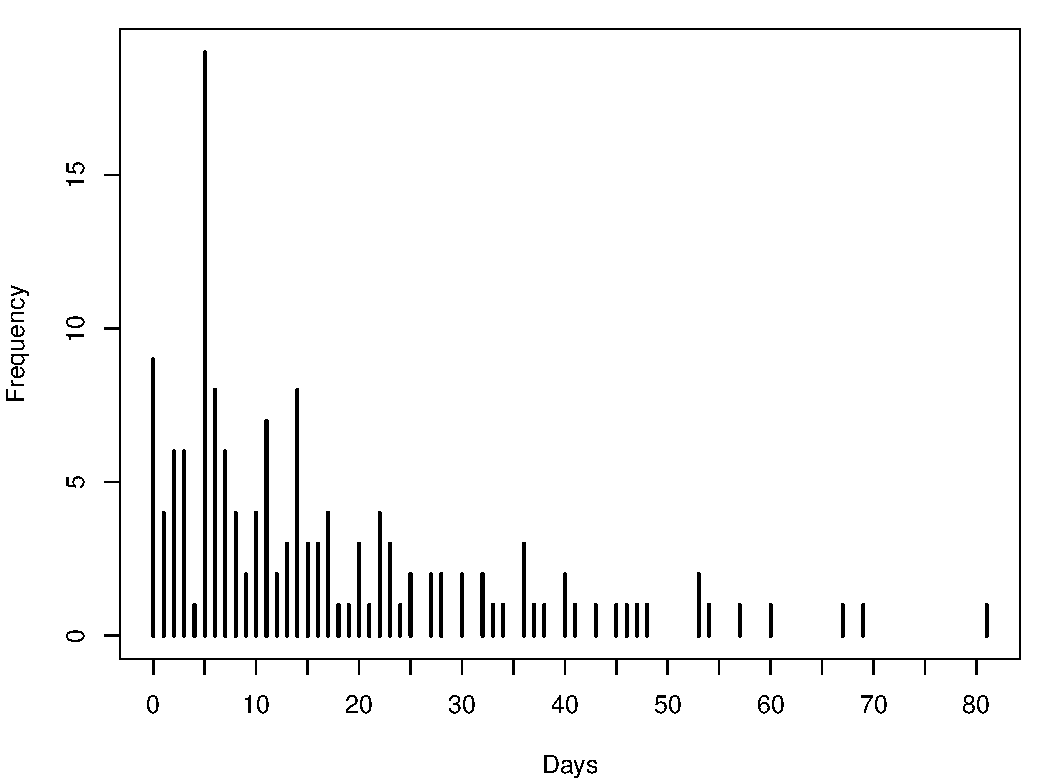
\includegraphics{article-visualization.pdf}

}

\caption{\label{fig-quine}Frequency distribution for number of days
absent from school.}

\end{figure}%

As a first model for the \texttt{quine} data, we fit the basic Poisson
regression model. (Note that JSS prefers when the second line of code is
indented by two spaces.)

\begin{verbatim}
R> m_pois <- glm(Days ~ (Eth + Sex + Age + Lrn)^2, data = quine, family = poisson)
\end{verbatim}

To account for potential overdispersion we also consider a negative
binomial GLM.

\begin{verbatim}
R> library("MASS")
R> m_nbin <- glm.nb(Days ~ (Eth + Sex + Age + Lrn)^2, data = quine)
\end{verbatim}

In a comparison with the BIC the latter model is clearly preferred.

\begin{verbatim}
R> library("MASS")
R> BIC(m_pois, m_nbin)
\end{verbatim}

\begin{verbatim}
       df      BIC
m_pois 18 2046.851
m_nbin 19 1157.235
\end{verbatim}

Hence, the full summary of that model is shown below.

\begin{verbatim}
R> summary(m_nbin)
\end{verbatim}

\begin{verbatim}

Call:
glm.nb(formula = Days ~ (Eth + Sex + Age + Lrn)^2, data = quine, 
    init.theta = 1.60364105, link = log)

Coefficients: (1 not defined because of singularities)
            Estimate Std. Error z value Pr(>|z|)    
(Intercept)  3.00155    0.33709   8.904  < 2e-16 ***
EthN        -0.24591    0.39135  -0.628  0.52977    
SexM        -0.77181    0.38021  -2.030  0.04236 *  
AgeF1       -0.02546    0.41615  -0.061  0.95121    
AgeF2       -0.54884    0.54393  -1.009  0.31296    
AgeF3       -0.25735    0.40558  -0.635  0.52574    
LrnSL        0.38919    0.48421   0.804  0.42153    
EthN:SexM    0.36240    0.29430   1.231  0.21818    
EthN:AgeF1  -0.70000    0.43646  -1.604  0.10876    
EthN:AgeF2  -1.23283    0.42962  -2.870  0.00411 ** 
EthN:AgeF3   0.04721    0.44883   0.105  0.91622    
EthN:LrnSL   0.06847    0.34040   0.201  0.84059    
SexM:AgeF1   0.02257    0.47360   0.048  0.96198    
SexM:AgeF2   1.55330    0.51325   3.026  0.00247 ** 
SexM:AgeF3   1.25227    0.45539   2.750  0.00596 ** 
SexM:LrnSL   0.07187    0.40805   0.176  0.86019    
AgeF1:LrnSL -0.43101    0.47948  -0.899  0.36870    
AgeF2:LrnSL  0.52074    0.48567   1.072  0.28363    
AgeF3:LrnSL       NA         NA      NA       NA    
---
Signif. codes:  0 '***' 0.001 '**' 0.01 '*' 0.05 '.' 0.1 ' ' 1

(Dispersion parameter for Negative Binomial(1.6036) family taken to be 1)

    Null deviance: 235.23  on 145  degrees of freedom
Residual deviance: 167.53  on 128  degrees of freedom
AIC: 1100.5

Number of Fisher Scoring iterations: 1

              Theta:  1.604 
          Std. Err.:  0.214 

 2 x log-likelihood:  -1062.546 
\end{verbatim}

\section{Summary and discussion}\label{sec-summary}

\begin{tcolorbox}[enhanced jigsaw, colframe=quarto-callout-color-frame, leftrule=.75mm, breakable, left=2mm, bottomrule=.15mm, toprule=.15mm, opacityback=0, colback=white, arc=.35mm, rightrule=.15mm]

As usual\ldots{}

\end{tcolorbox}

\section*{Computational details}\label{computational-details}
\addcontentsline{toc}{section}{Computational details}

\begin{tcolorbox}[enhanced jigsaw, colframe=quarto-callout-color-frame, leftrule=.75mm, breakable, left=2mm, bottomrule=.15mm, toprule=.15mm, opacityback=0, colback=white, arc=.35mm, rightrule=.15mm]

If necessary or useful, information about certain computational details
such as version numbers, operating systems, or compilers could be
included in an unnumbered section. Also, auxiliary packages (say, for
visualizations, maps, tables, \ldots) that are not cited in the main
text can be credited here.

\end{tcolorbox}

The results in this paper were obtained using
\proglang{R}\textasciitilde3.4.1 with the
\pkg{MASS}\textasciitilde7.3.47 package. \proglang{R} itself and all
packages used are available from the Comprehensive \proglang{R} Archive
Network (CRAN) at {[}https://CRAN.R-project.org/{]}.

\section*{Acknowledgments}\label{acknowledgments}
\addcontentsline{toc}{section}{Acknowledgments}

\begin{tcolorbox}[enhanced jigsaw, colframe=quarto-callout-color-frame, leftrule=.75mm, breakable, left=2mm, bottomrule=.15mm, toprule=.15mm, opacityback=0, colback=white, arc=.35mm, rightrule=.15mm]

All acknowledgments (note the AE spelling) should be collected in this
unnumbered section before the references. It may contain the usual
information about funding and feedback from colleagues/reviewers/etc.
Furthermore, information such as relative contributions of the authors
may be added here (if any).

\end{tcolorbox}

\section*{References}\label{references}
\addcontentsline{toc}{section}{References}

\renewcommand{\bibsection}{}
\bibliography{bibliography.bib}

\newpage{}

\section*{More technical details}\label{sec-techdetails}
\addcontentsline{toc}{section}{More technical details}

\begin{tcolorbox}[enhanced jigsaw, colframe=quarto-callout-color-frame, leftrule=.75mm, breakable, left=2mm, bottomrule=.15mm, toprule=.15mm, opacityback=0, colback=white, arc=.35mm, rightrule=.15mm]

Appendices can be included after the bibliography (with a page break).
Each section within the appendix should have a proper section title
(rather than just \emph{Appendix}).

For more technical style details, please check out JSS's style FAQ at
{[}https://www.jstatsoft.org/pages/view/style\#frequently-asked-questions{]}
which includes the following topics:

\begin{itemize}
\tightlist
\item
  Title vs.~sentence case.
\item
  Graphics formatting.
\item
  Naming conventions.
\item
  Turning JSS manuscripts into \proglang{R} package vignettes.
\item
  Trouble shooting.
\item
  Many other potentially helpful details\ldots{}
\end{itemize}

\end{tcolorbox}

\section*{Using BibTeX}\label{sec-bibtex}
\addcontentsline{toc}{section}{Using BibTeX}

\begin{tcolorbox}[enhanced jigsaw, colframe=quarto-callout-color-frame, leftrule=.75mm, breakable, left=2mm, bottomrule=.15mm, toprule=.15mm, opacityback=0, colback=white, arc=.35mm, rightrule=.15mm]

References need to be provided in a \textsc{Bib}{\TeX} file
(\texttt{.bib}). All references should be made with \texttt{@cite}
syntax. This commands yield different formats of author-year citations
and allow to include additional details (e.g.,pages, chapters, \dots) in
brackets. In case you are not familiar with these commands see the JSS
style FAQ for details.

Cleaning up \textsc{Bib}{\TeX} files is a somewhat tedious task --
especially when acquiring the entries automatically from mixed online
sources. However, it is important that informations are complete and
presented in a consistent style to avoid confusions. JSS requires the
following format.

\begin{itemize}
\tightlist
\item
  item JSS-specific markup (\texttt{\textbackslash{}proglang},
  \texttt{\textbackslash{}pkg}, \texttt{\textbackslash{}code}) should be
  used in the references.
\item
  item Titles should be in title case.
\item
  item Journal titles should not be abbreviated and in title case.
\item
  item DOIs should be included where available.
\item
  item Software should be properly cited as well. For \proglang{R}
  packages \texttt{citation("pkgname")} typically provides a good
  starting point.
\end{itemize}

\end{tcolorbox}




\end{document}
